\documentclass[12pt,a4paper]{article}

% Packages
\usepackage[utf8]{inputenc}
\usepackage[vietnamese]{babel}
\usepackage{geometry}
\usepackage{graphicx}
\usepackage{hyperref}
\usepackage{listings}
\usepackage{xcolor}
\usepackage{amsmath}
\usepackage{float}
\usepackage{caption}
\usepackage{subcaption}
\usepackage{enumitem}
\usepackage{fancyhdr}
\usepackage{titlesec}
\usepackage{tocloft}

% Page geometry
\geometry{
    left=3cm,
    right=2cm,
    top=2.5cm,
    bottom=2.5cm
}

% Header and footer
\pagestyle{fancy}
\fancyhf{}
\fancyhead[L]{Vending Machine System}
\fancyhead[R]{STM32 Project Report}
\fancyfoot[C]{\thepage}

% Code listing style
\lstdefinestyle{cstyle}{
    language=C,
    basicstyle=\ttfamily\small,
    keywordstyle=\color{blue}\bfseries,
    commentstyle=\color{gray}\itshape,
    stringstyle=\color{red},
    numbers=left,
    numberstyle=\tiny\color{gray},
    stepnumber=1,
    numbersep=8pt,
    backgroundcolor=\color{white},
    showspaces=false,
    showstringspaces=false,
    showtabs=false,
    frame=single,
    rulecolor=\color{black},
    tabsize=4,
    captionpos=b,
    breaklines=true,
    breakatwhitespace=false,
    escapeinside={(*@}{@*)}
}

\lstset{style=cstyle}

% Hyperref setup
\hypersetup{
    colorlinks=true,
    linkcolor=black,
    citecolor=blue,
    urlcolor=blue,
    pdftitle={Vending Machine Technical Report},
    pdfauthor={Nguyen Hung Thinh, Le The Loc, Tran Doan Hoang Lam}
}

% Title information
\title{
    \Large\textbf{TRƯỜNG ĐẠI HỌC BÁCH KHOA TP.HCM}\\
    \large Khoa Khoa học và Kỹ thuật Máy tính\\
    \vspace{0.5cm}
    \includegraphics[width=8cm]{../Pictures/hcmut.png}\\
    \rule{\textwidth}{1.5pt}\\
    \vspace{0.5cm}
    \Huge\textbf{MÁY BÁN HÀNG TỰ ĐỘNG}\\
    \Large\textbf{Báo cáo Kỹ thuật}\\
    \vspace{0.3cm}
    \Large Đồ án Thiết kế Luận lý với Vi điều khiển STM32\\
    \rule{\textwidth}{1.5pt}\\
}

\author{
    \textbf{Giảng viên hướng dẫn:}\\
    Nguyễn Thành Lộc\\
    \vspace{1cm}\\
    \textbf{Nhóm tác giả:}\\
    Nguyễn Hưng Thịnh\\
    Lê Thế Lộc\\
    Trần Doãn Hoàng Lâm\\
    \vspace{1cm}\\
    \textbf{Đơn vị:}\\
    Trường Đại học Bách Khoa TP.HCM (HCMUT)\\
}

% Get current date in Vietnamese format automatically
\date{\today}

\begin{document}

% Title page
\maketitle
\thispagestyle{empty}
\newpage

% Abstract
\begin{abstract}
Báo cáo kỹ thuật này trình bày quá trình thiết kế 
và hiện thực hệ thống máy bán hàng tự động thông minh 
sử dụng vi điều khiển STM32F103C8T6. 
Hệ thống được thiết kế đặc biệt để bán các vật phẩm trong trò chơi 
(Trang phục đội tuyển SKT trong Liên Minh Huyền Thoại) và có các tính năng 
như tự động phát hiện khách hàng thông qua cảm biến siêu âm, 
giao diện LCD tương tác với bàn phím, 
quản lý kho hàng sử dụng bộ nhớ Flash, 
xử lý thanh toán toàn diện 
và chế độ quản trị bảo mật để kiểm soát kho hàng. 
Dự án minh họa các ứng dụng thực tế của 
nguyên lý hệ thống nhúng bao gồm thiết kế 
máy trạng thái hữu hạn, giao tiếp ngoại vi, 
điều khiển thời gian thực và lưu trữ dữ liệu. 
Việc hiện thực sử dụng thư viện STM32 HAL và 
bao gồm các trình điều khiển tùy chỉnh cho giao tiếp LCD I2C, 
quét bàn phím ma trận 4x4 và đo khoảng cách siêu âm HC-SR04. 
Các tính năng chính bao gồm tự động bật nguồn thông qua đo khoảng cách, 
xử lý giao dịch đa trạng thái với xử lý lỗi và lưu trữ kho hàng 
dựa trên bộ nhớ Flash.
\end{abstract}

\newpage

% Table of contents
\renewcommand{\contentsname}{Mục lục}
\tableofcontents
\newpage

% Main content
\newpage
\section{Tổng quan Hệ thống}

\subsection{Kiến trúc Hệ thống}

Hệ thống máy bán hàng tự động tuân theo mẫu thiết kế kiến trúc phân lớp, tách biệt phần trừu tượng hóa phần cứng, logic nghiệp vụ và giao diện người dùng. Hình \ref{fig:system_architecture} minh họa kiến trúc tổng thể của hệ thống.

\begin{figure}[H]
    \centering
    \includegraphics[width=0.9\textwidth]{../Pictures/architecture.png}
    \caption{Sơ đồ kiến trúc hệ thống}
    \label{fig:system_architecture}
\end{figure}

Kiến trúc bao gồm bốn lớp chính:

\subsubsection{Lớp Phần cứng}

Lớp này bao gồm tất cả các thành phần vật lý và giao diện phần cứng cấp thấp:

\begin{itemize}[leftmargin=*]
    \item \textbf{Vi điều khiển STM32F103C8T6:} Đơn vị xử lý trung tâm quản lý mọi hoạt động, chạy ở tần số 72 MHz với lõi ARM Cortex-M3
    \item \textbf{Màn hình LCD I2C:} Màn hình ký tự 16x2 kết nối qua bộ mở rộng I2C PCF8574 trên các chân PB6 (SCL) và PB7 (SDA)
    \item \textbf{Bàn phím ma trận 4x4:} Thiết bị đầu vào với các hàng trên PA0-PA3 và các cột trên PA4-PA7
    \item \textbf{Cảm biến siêu âm HC-SR04:} Mô-đun đo khoảng cách sử dụng bộ bắt đầu vào TIM1 để định thời chính xác
    \item \textbf{Bộ nhớ Flash:} Flash nội bộ 64KB với Trang 63 được dành riêng để lưu trữ dữ liệu
    \item \textbf{Đèn báo LED:} LED tích hợp trên PC13 để chỉ báo trạng thái hệ thống
\end{itemize}

\subsubsection{Lớp Trình điều khiển}

Các trình điều khiển ngoại vi tùy chỉnh cung cấp sự trừu tượng hóa phần cứng:

\begin{itemize}[leftmargin=*]
    \item \textbf{Trình điều khiển LCD I2C (tv\_lcd\_i2c.c):} Hiện thực giao tiếp LCD 4-bit qua giao thức I2C bit-banged
    \item \textbf{Trình điều khiển Bàn phím (keypad.c):} Cung cấp chức năng quét, chống rung và ánh xạ ký tự
    \item \textbf{Trình điều khiển Cảm biến (sensor.c):} Xử lý kích hoạt siêu âm và tính toán khoảng cách thông qua bộ bắt thời gian
    \item \textbf{Trình điều khiển I2C (i2c.c):} Hiện thực giao thức I2C dựa trên phần mềm để giao tiếp LCD
    \item \textbf{Quản lý Bộ định thời (timer.c):} Hệ thống định thời phần mềm cho các thời gian chờ và độ trễ trạng thái
\end{itemize}

\subsubsection{Lớp Ứng dụng}

Logic nghiệp vụ và quản lý trạng thái:

\begin{itemize}[leftmargin=*]
    \item \textbf{Máy trạng thái hữu hạn (fsm\_vm.c):} Logic cốt lõi với 19 trạng thái quản lý luồng giao dịch, xử lý lỗi và chuyển đổi chế độ
    \item \textbf{Quản lý Kho hàng (store.c):} Xử lý cấu trúc dữ liệu sản phẩm, thao tác đọc/ghi Flash và cập nhật tồn kho
    \item \textbf{Mô-đun Quản trị (ADMIN.c):} Xác thực mật khẩu và quản lý bảo mật
\end{itemize}

\subsubsection{Lớp Giao diện Người dùng}

Quản lý trình bày và tương tác:

\begin{itemize}[leftmargin=*]
    \item Định dạng hiển thị LCD và trình bày văn bản căn giữa
    \item Thông dịch đầu vào bàn phím và ánh xạ lệnh
    \item Phản hồi trạng thái và hiển thị thông báo lỗi
    \item Luồng điều hướng đa màn hình
\end{itemize}

\subsection{Triết lý Thiết kế}

Thiết kế hệ thống tuân theo một số nguyên tắc chính:

\subsubsection{Tính Mô-đun và Phân tách Mối quan tâm}

Mỗi thành phần chức năng được hiện thực như một mô-đun độc lập với các giao diện được xác định rõ. Ví dụ, trình điều khiển LCD cung cấp các hàm cấp cao như \texttt{lcd\_write\_string()} mà không để lộ chi tiết giao tiếp I2C. Tính mô-đun này tạo điều kiện thuận lợi cho việc kiểm tra, gỡ lỗi và sửa đổi trong tương lai.

\subsubsection{Kiến trúc Hướng Trạng thái}

Hệ thống sử dụng máy trạng thái hữu hạn làm cấu trúc điều khiển cốt lõi, cung cấp:

\begin{itemize}[leftmargin=*]
    \item \textbf{Hành vi Dự đoán được:} Mỗi trạng thái có các điều kiện đầu vào, hành động và chuyển đổi đầu ra được xác định
    \item \textbf{Phục hồi Lỗi:} Các trạng thái lỗi cho phép xử lý nhẹ nhàng các đầu vào không hợp lệ và điều kiện thời gian chờ
    \item \textbf{Khả năng Bảo trì:} Thêm các tính năng mới đòi hỏi thêm các trạng thái và chuyển đổi mà không cần cấu trúc lại mã hiện có
    \item \textbf{Gỡ lỗi:} Theo dõi biến trạng thái đơn giản hóa việc phân tích hành vi hệ thống
\end{itemize}

\subsubsection{Vận hành An toàn}

Nhiều cơ chế an toàn đảm bảo độ tin cậy của hệ thống:

\begin{itemize}[leftmargin=*]
    \item Bộ định thời gian chờ ngăn chặn việc chờ đợi vô thời hạn (30 giây cho khách hàng, 60 giây cho quản trị viên)
    \item Bộ đếm lỗi giới hạn các lỗi liên tiếp (tối đa 5 lần thử)
    \item Kiểm tra đầu vào từ chối số lượng và số tiền thanh toán không hợp lệ
    \item Xác minh số ma thuật Flash ngăn chặn việc tải dữ liệu bị hỏng
\end{itemize}

\subsubsection{Thiết kế Lấy Người dùng làm Trung tâm}

Giao diện ưu tiên trải nghiệm người dùng thông qua:

\begin{itemize}[leftmargin=*]
    \item Điều hướng rõ ràng với các ánh xạ phím nhất quán (U/D để điều hướng, \# để xác nhận, * để quay lại)
    \item Phản hồi ngay lập tức cho mọi hành động của người dùng
    \item Hiển thị văn bản căn giữa để cải thiện khả năng đọc
    \item Thông báo lỗi cung cấp thông tin với hướng dẫn phục hồi
    \item Tự động quay lại trạng thái an toàn khi hết thời gian chờ
\end{itemize}

\subsection{Yêu cầu Hệ thống}

\begin{enumerate}[label=FR\arabic*:, leftmargin=*]
    \item \textbf{Phát hiện Khách hàng:} Hệ thống sẽ phát hiện sự hiện diện của khách hàng trong phạm vi 20cm trong 3 giây liên tiếp và tự động bật nguồn
    
    \item \textbf{Duyệt Sản phẩm:} Người dùng sẽ điều hướng qua 16 sản phẩm bằng các phím Lên/Xuống với cập nhật hiển thị thời gian thực
    
    \item \textbf{Thông tin Sản phẩm:} Hệ thống sẽ hiển thị tên sản phẩm, tên người chơi, số lượng có sẵn và giá
    
    \item \textbf{Chọn Số lượng:} Người dùng sẽ nhập số lượng từ 1-9 đơn vị với xác thực và phản hồi lỗi
    
    \item \textbf{Xử lý Thanh toán:} Hệ thống sẽ chấp nhận các mệnh giá tiền tệ Việt Nam (5K, 10K, 20K, 50K, 100K, 200K, 500K VND) và tính toán tiền thừa
    
    \item \textbf{Quản lý Kho hàng:} Hệ thống sẽ theo dõi mức tồn kho và ngăn chặn bán hàng khi hết hàng
    
    \item \textbf{Lưu trữ Dữ liệu:} Dữ liệu kho hàng sẽ tồn tại qua các chu kỳ nguồn sử dụng bộ nhớ Flash
    
    \item \textbf{Truy cập Quản trị:} Chế độ quản trị được bảo vệ bằng mật khẩu sẽ cho phép điều chỉnh kho hàng và giá cả
    
    \item \textbf{Xử lý Lỗi:} Hệ thống sẽ xử lý các đầu vào không hợp lệ, thời gian chờ và hiển thị các thông báo lỗi thích hợp
    
    \item \textbf{Hoàn tất Giao dịch:} Khi thanh toán thành công, hệ thống sẽ cập nhật kho hàng và quay lại lựa chọn sản phẩm
\end{enumerate}

\subsection{Luồng Vận hành Hệ thống}

Hoạt động hoàn chỉnh của hệ thống tuân theo trình tự sau:

\begin{enumerate}[leftmargin=*]
    \item \textbf{Giai đoạn Khởi tạo:}
    \begin{itemize}
        \item Bật nguồn và khởi tạo phần cứng
        \item Tải kho hàng từ bộ nhớ Flash (hoặc khởi tạo mặc định nếu là lần khởi động đầu tiên)
        \item Cấu hình tất cả các thiết bị ngoại vi (GPIO, I2C, Timer)
        \item Hiển thị màn hình khởi tạo
        \item Vào trạng thái nhàn rỗi với giám sát cảm biến
    \end{itemize}
    
    \item \textbf{Giai đoạn Phát hiện Khách hàng:}
    \begin{itemize}
        \item Quét liên tục cảm biến siêu âm mỗi 100ms
        \item Phát hiện sự hiện diện khi khoảng cách $\leq$ 20cm trong 3 giây
        \item Kích hoạt đèn nền và hiển thị thông báo chào mừng
        \item Chuyển sang chế độ chọn sản phẩm
    \end{itemize}
    
    \item \textbf{Giai đoạn Chọn Sản phẩm:}
    \begin{itemize}
        \item Hiển thị sản phẩm hiện tại (ID, tên, người chơi)
        \item Chấp nhận các phím Lên/Xuống để điều hướng qua 16 sản phẩm
        \item Phím \# để xem thông tin chi tiết
        \item Phím R để vào chế độ quản trị (yêu cầu mật khẩu)
        \item Thời gian chờ không hoạt động 30 giây quay lại trạng thái nhàn rỗi
    \end{itemize}
    
    \item \textbf{Giai đoạn Mua hàng:}
    \begin{itemize}
        \item Hiển thị chi tiết số lượng và giá
        \item Chấp nhận đầu vào số lượng (1-9 đơn vị)
        \item Xác thực tình trạng còn hàng
        \item Tính toán và hiển thị tổng số tiền thanh toán
        \item Chấp nhận đầu vào thanh toán với xác thực mệnh giá
        \item Tính toán tiền thừa nếu trả thừa
        \item Cập nhật kho hàng và lưu vào Flash
    \end{itemize}
    
    \item \textbf{Giai đoạn Chế độ Quản trị:}
    \begin{itemize}
        \item Xác thực với mật khẩu 6 chữ số
        \item Điều hướng sản phẩm để điều chỉnh
        \item Sửa đổi số lượng (0-9) và giá (1K-99K VND)
        \item Lưu thay đổi vào bộ nhớ Flash
        \item Thời gian chờ không hoạt động 60 giây để bảo mật
    \end{itemize}
\end{enumerate}

\newpage
\section{Thành phần Phần cứng}

Phần này cung cấp thông số kỹ thuật chi tiết và chi tiết tích hợp cho tất cả các thành phần phần cứng được sử dụng trong hệ thống máy bán hàng tự động.

\begin{figure}[H]
    \centering
    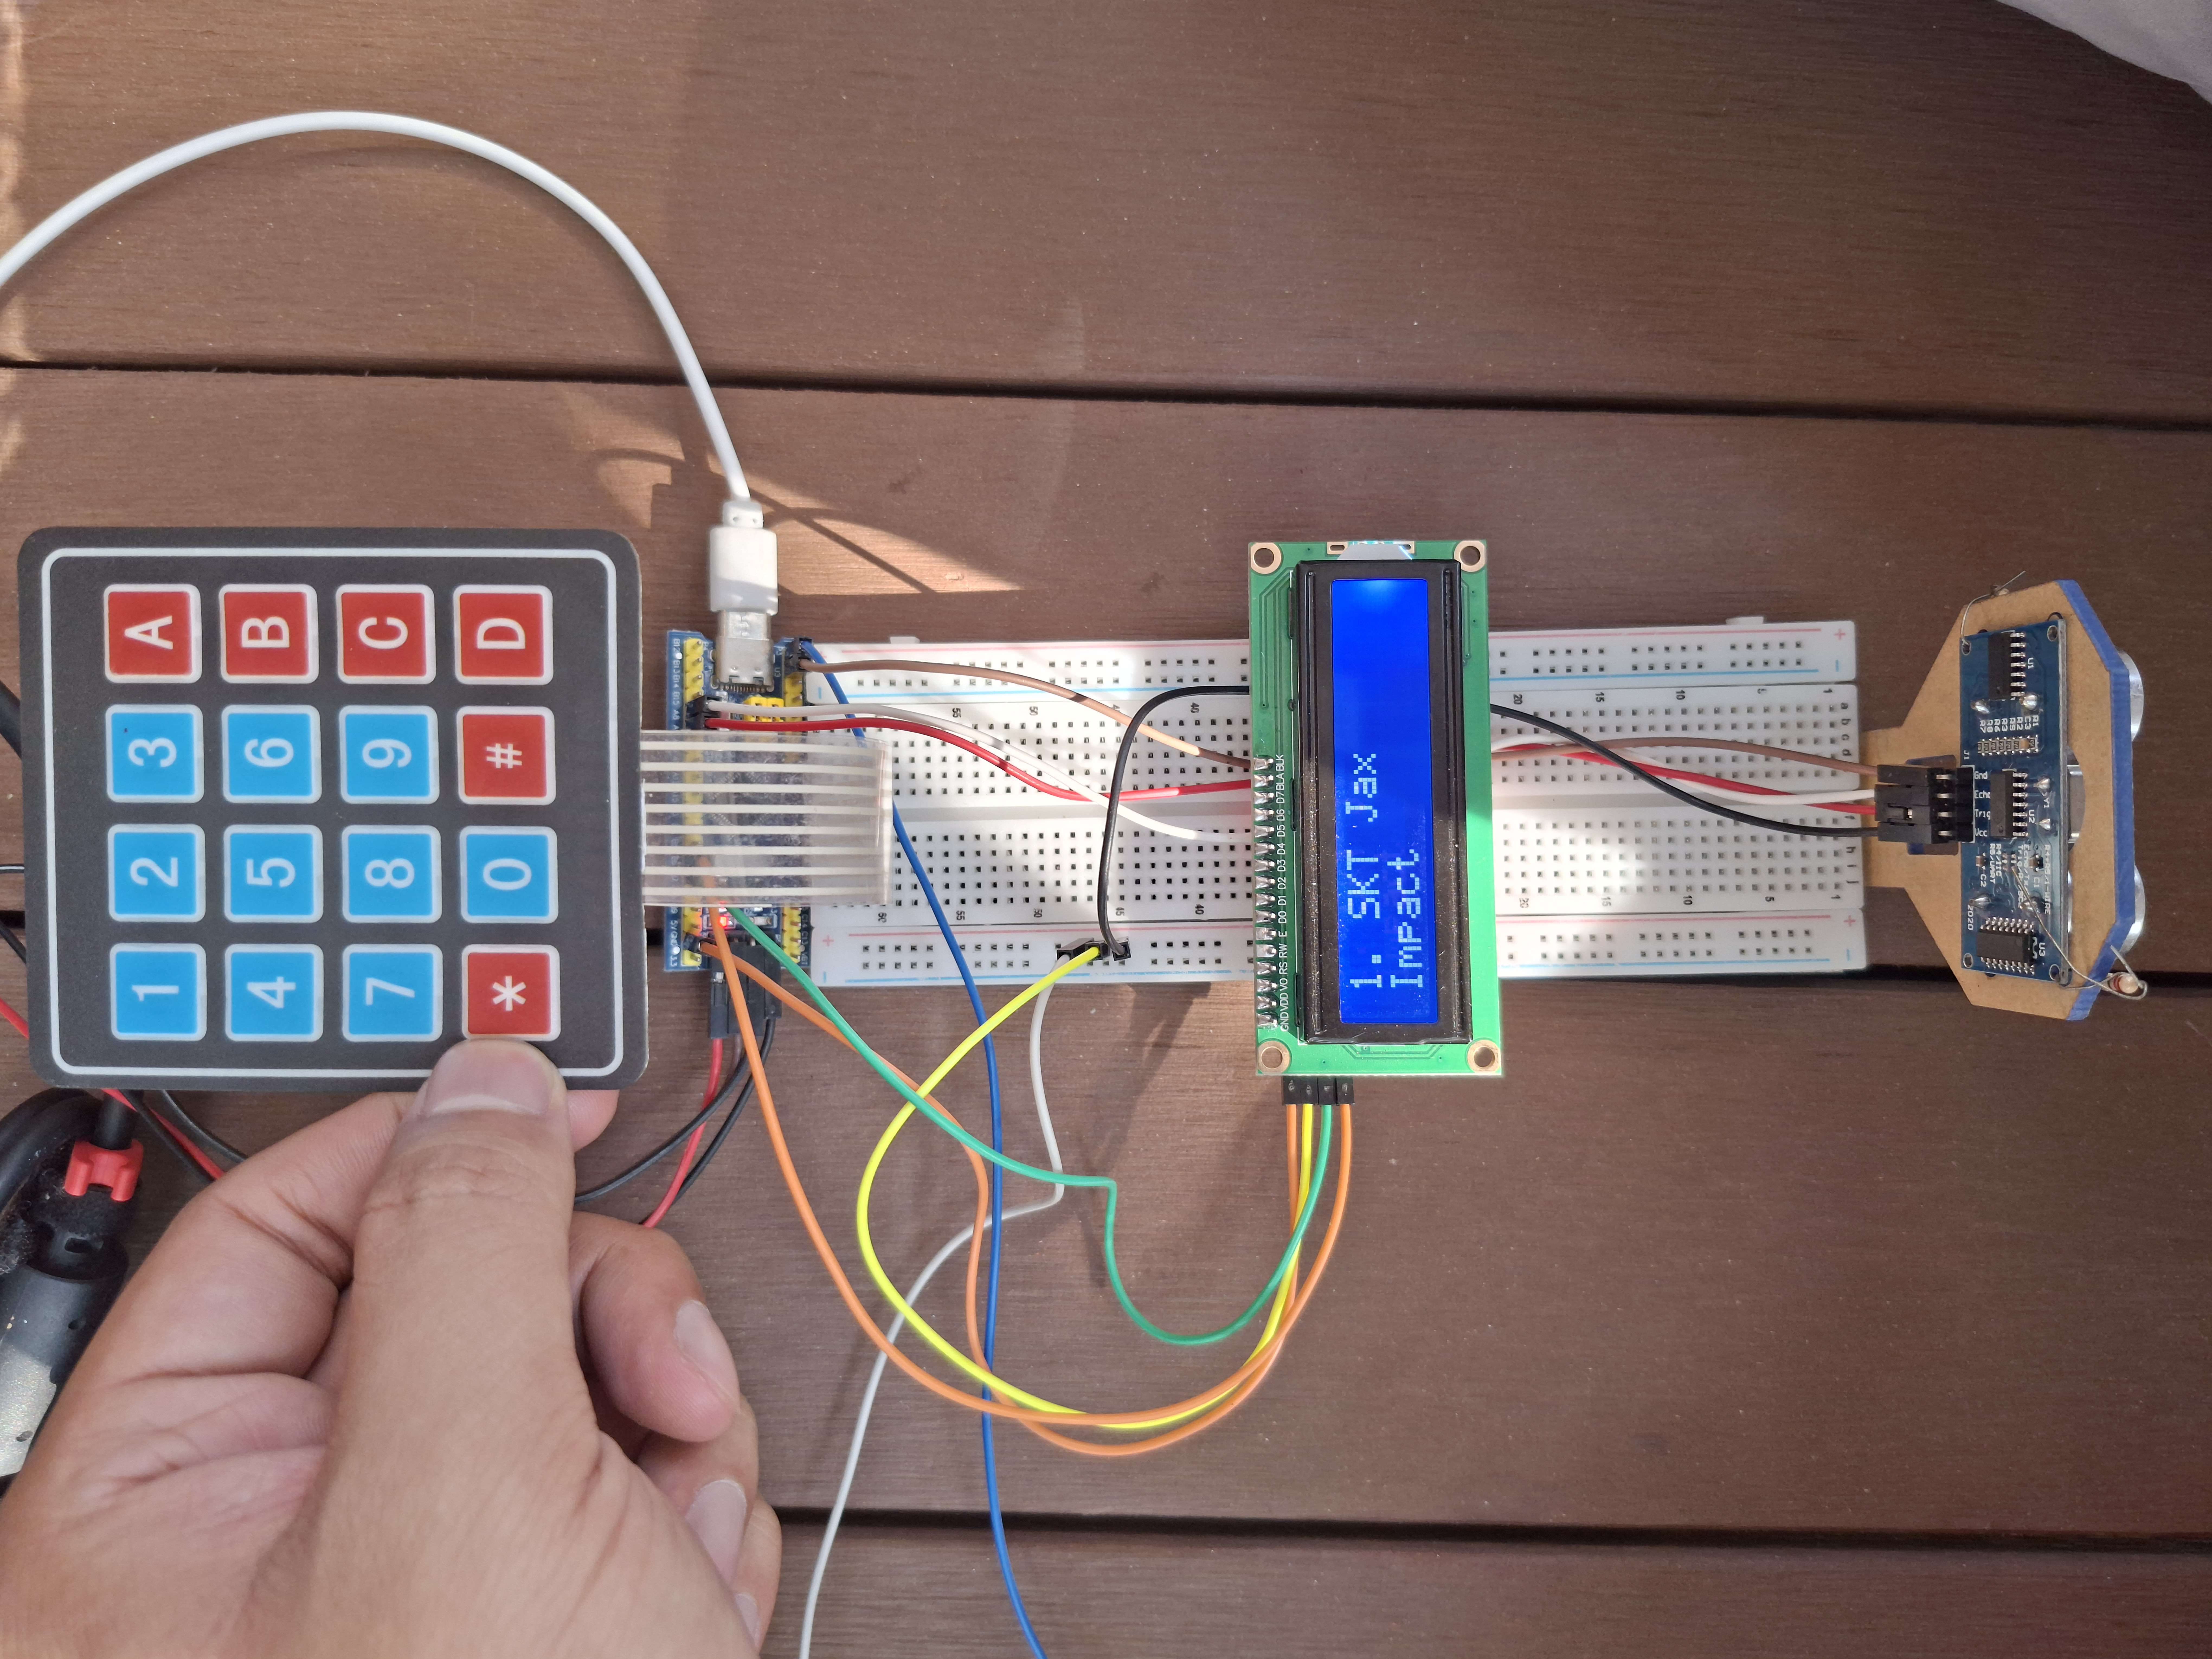
\includegraphics[width=0.9\textwidth]{../Pictures/topView.jpg}
    \caption{Hiện thực phần cứng của hệ thống Máy bán hàng tự động}
    \label{fig:hardware_overview}
\end{figure}

\subsection{Vi điều khiển - STM32F103C8T6}

STM32F103C8T6 (thường được gọi là "Blue Pill") đóng vai trò là đơn vị xử lý trung tâm của hệ thống.

\subsubsection{Lý do Lựa chọn}

STM32F103C8T6 được chọn cho dự án này vì:

\begin{itemize}[leftmargin=*]
    \item \textbf{Sức mạnh Xử lý:} Xung nhịp 72 MHz cung cấp đủ hiệu năng cho các hoạt động thời gian thực
    \item \textbf{Bộ nhớ:} 64 KB Flash chứa được các trình điều khiển HAL và mã ứng dụng; 20 KB RAM đủ cho dữ liệu thời gian chạy
    \item \textbf{Hỗ trợ Ngoại vi:} Tích hợp sẵn I2C, bộ định thời và GPIO đáp ứng mọi yêu cầu giao diện
    \item \textbf{Hệ sinh thái Phát triển:} Hỗ trợ tuyệt vời thông qua STM32CubeIDE và thư viện HAL
    \item \textbf{Hiệu quả Chi phí:} Bo mạch phát triển giá rẻ có sẵn rộng rãi
    \item \textbf{Hỗ trợ Cộng đồng:} Cộng đồng người dùng lớn và tài liệu phong phú
\end{itemize}

\subsubsection{Cấu hình Chân}

Các gán chân quan trọng cho dự án này:

\begin{table}[H]
\centering
\caption{Gán chân STM32F103C8T6}
\begin{tabular}{|l|l|l|}
\hline
\textbf{Chân} & \textbf{Chức năng} & \textbf{Mô tả} \\
\hline
PA0-PA3 & Hàng Bàn phím & Chân đầu ra để quét bàn phím \\
PA4-PA7 & Cột Bàn phím & Chân đầu vào với điện trở kéo lên \\
PB6 & I2C1\_SCL & Xung nhịp I2C cho giao tiếp LCD \\
PB7 & I2C1\_SDA & Dữ liệu I2C cho giao tiếp LCD \\
PA8 & TIM1\_CH1 & ECHO cảm biến siêu âm (Bắt đầu vào) \\
PA9 & GPIO Output & TRIG cảm biến siêu âm \\
PC13 & GPIO Output & Đèn báo LED (tích cực mức thấp) \\
PA13 & SWDIO & Dữ liệu I/O Gỡ lỗi Serial Wire \\
PA14 & SWCLK & Xung nhịp Gỡ lỗi Serial Wire \\
\hline
\end{tabular}
\end{table}

\subsection{Mô-đun Hiển thị - LCD 16x2 với I2C}

Hệ thống sử dụng màn hình LCD 16x2 kết hợp với bộ mở rộng I/O I2C PCF8574 để hiển thị thông tin.

\subsubsection{Giao thức Giao tiếp}

Hệ thống hiện thực giao tiếp I2C bit-banged:

\begin{enumerate}[leftmargin=*]
    \item \textbf{Điều kiện START:} SDA chuyển từ cao xuống thấp trong khi SCL ở mức cao
    \item \textbf{Khung Địa chỉ:} Gửi địa chỉ slave 7-bit + bit R/W
    \item \textbf{Truyền Dữ liệu:} Gửi dữ liệu 8-bit với kiểm tra ACK
    \item \textbf{Điều kiện STOP:} SDA chuyển từ thấp lên cao trong khi SCL ở mức cao
\end{enumerate}

Đối với hoạt động LCD ở chế độ 4-bit:
\begin{enumerate}[leftmargin=*]
    \item Gửi nibble cao (4 bit) của byte dữ liệu
    \item Tạo xung chân Enable
    \item Gửi nibble thấp (4 bit) của byte dữ liệu
    \item Tạo xung chân Enable
\end{enumerate}

\subsection{Thiết bị Đầu vào - Bàn phím Ma trận 4×4}

Bàn phím ma trận cung cấp 16 phím được sắp xếp thành 4 hàng và 4 cột, hoạt động dựa trên nguyên tắc quét hàng-cột.

\subsubsection{Chiến lược Chống rung}

Các công tắc cơ học thể hiện hiện tượng rung, gây ra nhiều chuyển đổi trong một lần nhấn. Hệ thống hiện thực chống rung bằng phần mềm:

\begin{lstlisting}[language=C, caption={Hiện thực Chống rung Bàn phím}]
if (HAL_GPIO_ReadPin(GPIOA, col_pins[c]) == GPIO_PIN_RESET) {
    HAL_Delay(20); // Debounce delay
    
    if (HAL_GPIO_ReadPin(GPIOA, col_pins[c]) == GPIO_PIN_RESET) {
        // Key press confirmed
        while (HAL_GPIO_ReadPin(GPIOA, col_pins[c]) == GPIO_PIN_RESET);
        // Wait for release
        return keymap[r][c];
    }
}
\end{lstlisting}

\subsection{Mô-đun Cảm biến - Cảm biến Siêu âm HC-SR04}

HC-SR04 sử dụng phép đo thời gian bay (time-of-flight) để đo khoảng cách.

\subsubsection{Cấu hình Bắt đầu vào Bộ định thời}

Hệ thống sử dụng Kênh 1 của TIM1 được cấu hình cho chế độ Bắt đầu vào (Input Capture):

\begin{itemize}[leftmargin=*]
    \item \textbf{Chế độ Bắt:} Cả hai cạnh (lên và xuống)
    \item \textbf{Tần số Bộ định thời:} 1 MHz (độ phân giải 1 micro giây)
    \item \textbf{Ngắt:} Được kích hoạt khi có sự kiện bắt
\end{itemize}

Trình tự đo:
\begin{enumerate}[leftmargin=*]
    \item Bắt lần đầu (cạnh lên): Ghi lại thời gian bắt đầu IC\_Val1
    \item Bắt lần hai (cạnh xuống): Ghi lại thời gian kết thúc IC\_Val2
    \item Tính hiệu số: $Difference = IC\_Val2 - IC\_Val1$
    \item Xử lý tràn bộ định thời: Nếu $IC\_Val1 > IC\_Val2$, cộng thêm chu kỳ bộ định thời
    \item Chuyển đổi sang khoảng cách: $Distance = Difference \times 0.034 / 2$
\end{enumerate}

\subsection{Bộ nhớ - Flash Nội bộ}

Hệ thống sử dụng trang cuối cùng (Trang 63) của bộ nhớ Flash nội bộ để lưu trữ dữ liệu kho hàng, đảm bảo dữ liệu được bảo toàn khi mất điện.

\subsubsection{Chiến lược Bảo toàn Dữ liệu}

Cấu trúc dữ liệu kho hàng (44 byte mỗi sản phẩm):
\begin{itemize}[leftmargin=*]
    \item \textbf{Số Ma thuật:} 4 byte (0xDEADBEEF) để xác thực dữ liệu
    \item \textbf{Mảng Sản phẩm:} 16 sản phẩm × 44 byte = 704 byte
    \item \textbf{Tổng Lưu trữ:} 708 byte (vừa trong trang 1 KB)
\end{itemize}

Khi bật nguồn:
\begin{enumerate}[leftmargin=*]
    \item Đọc số ma thuật từ Trang 63 của Flash
    \item Nếu số ma thuật khớp 0xDEADBEEF: Tải kho hàng từ Flash
    \item Nếu số ma thuật không hợp lệ: Khởi tạo kho hàng mặc định và lưu vào Flash
\end{enumerate}

\subsection{Nguồn điện và Giao diện Lập trình}

\subsubsection{Yêu cầu Nguồn điện}

\begin{itemize}[leftmargin=*]
    \item \textbf{Lõi STM32:} 3.3V, ~50mA
    \item \textbf{Mô-đun LCD:} 5V, ~30mA (không đèn nền), ~150mA (có đèn nền)
    \item \textbf{Cảm biến HC-SR04:} 5V, ~15mA
    \item \textbf{Bàn phím:} Tiêu thụ dòng không đáng kể
    \item \textbf{Tổng Hệ thống:} ~200mA ở 5V hoạt động điển hình
\end{itemize}

Phân phối nguồn:
\begin{itemize}[leftmargin=*]
    \item Bộ chuyển đổi ngoài 5V cung cấp cho các đường nguồn breadboard
    \item Bộ ổn áp 3.3V tích hợp (AMS1117-3.3) cấp nguồn cho STM32
    \item LCD và cảm biến kết nối trực tiếp với đường nguồn 5V
\end{itemize}

\subsubsection{Bộ nạp ST-Link V2}

\begin{itemize}[leftmargin=*]
    \item \textbf{Giao diện:} SWD (Serial Wire Debug)
    \item \textbf{Kết nối:}
    \begin{itemize}
        \item SWDIO → PA13
        \item SWCLK → PA14
        \item GND → GND
        \item 3.3V → 3.3V (optional for powering during debug)
    \end{itemize}
    \item \textbf{Tính năng:} Programming, debugging, real-time variable monitoring
\end{itemize}

\newpage
\section{Thiết kế Phần mềm}

\subsection{Kiến trúc Máy trạng thái Hữu hạn}

Cốt lõi của phần mềm máy bán hàng tự động là một máy trạng thái hữu hạn (FSM) với 19 trạng thái riêng biệt quản lý toàn bộ vòng đời giao dịch, xử lý lỗi và các chức năng quản trị. FSM cung cấp hành vi xác định và đơn giản hóa việc gỡ lỗi bằng cách làm cho trạng thái hệ thống rõ ràng tại mọi thời điểm.

\subsubsection{Định nghĩa Trạng thái}

Hệ thống hiện thực 19 trạng thái riêng biệt, được định nghĩa trong \texttt{fsm\_vm.h}, bao gồm các trạng thái khởi tạo, giao dịch khách hàng và chế độ quản trị.

\subsubsection{Phân loại Trạng thái}

19 trạng thái được tổ chức thành các danh mục chức năng:

\paragraph{Trạng thái Khởi tạo (1-2):}
\begin{itemize}[leftmargin=*]
    \item \textbf{INIT:} Khởi tạo hệ thống, thiết lập ngoại vi, tải kho hàng từ Flash
    \item \textbf{WAIT\_SENSOR:} Trạng thái nhàn rỗi với giám sát cảm biến siêu âm liên tục để phát hiện khách hàng
\end{itemize}

\paragraph{Trạng thái Giao dịch Khách hàng (3-14):}
\begin{itemize}[leftmargin=*]
    \item \textbf{WELCOME\_SECTION:} Hiển thị thông báo chào mừng trong 3 giây
    \item \textbf{CHOOSING\_SKIN:} Duyệt sản phẩm với điều hướng Lên/Xuống
    \item \textbf{DISPLAY\_INFO:} Hiển thị thông tin chi tiết sản phẩm (số lượng, giá)
    \item \textbf{CHOOSING\_QUANTITY:} Nhập số lượng (1-9)
    \item \textbf{OUT\_OF\_STOCK\_NOTIFICATION:} Cảnh báo khi sản phẩm đã chọn không có sẵn
    \item \textbf{QUANTITY\_ERROR:} Xử lý nhập số lượng không hợp lệ với thử lại
    \item \textbf{MAX\_ERROR\_STATE:} Hủy giao dịch sau 5 lỗi liên tiếp
    \item \textbf{PAYMENT\_SHOW\_TOTAL:} Hiển thị tổng số tiền phải trả
    \item \textbf{PAYMENT\_INPUT:} Chấp nhận các mệnh giá thanh toán
    \item \textbf{PAYMENT\_ERROR:} Xử lý số tiền thanh toán không hợp lệ
    \item \textbf{PAYMENT\_INFO\_WAIT:} Hiển thị số tiền còn lại hoặc tiền thừa
    \item \textbf{THANKS:} Thông báo cảm ơn và cập nhật kho hàng
\end{itemize}

\paragraph{Trạng thái Chế độ Quản trị (15-19):}
\begin{itemize}[leftmargin=*]
    \item \textbf{ADMIN\_MODE:} Xác nhận đăng nhập thành công
    \item \textbf{CHOOSING\_SKIN\_TO\_ADJUST:} Chọn sản phẩm để sửa đổi
    \item \textbf{TIMEOUT\_ADMIN\_MODE:} Tự động đăng xuất sau 60 giây không hoạt động
    \item \textbf{ADJUST\_QUANTITY\_AND\_PRICE:} Chỉnh sửa kho hàng và giá cả
    \item \textbf{CONFIRM\_EXIT\_ADMIN\_MODE:} Hộp thoại xác nhận đăng xuất
\end{itemize}

\subsubsection{Sơ đồ Chuyển đổi Trạng thái}

Các chuyển đổi trạng thái tuân theo các đường dẫn chính sau:

\begin{figure}[H]
    \centering
    \includegraphics[width=0.9\textwidth]{../Pictures/fsm.png}
    \caption{Sơ đồ chuyển đổi trạng thái FSM (Chế độ Người dùng)}
    \label{fig:fsm_diagram}
\end{figure}

\begin{figure}[H]
    \centering
    \includegraphics[width=0.9\textwidth]{../Pictures/fsmAdmin.png}
    \caption{Sơ đồ chuyển đổi trạng thái FSM (Chế độ Quản trị)}
    \label{fig:fsm_admin_diagram}
\end{figure}

\textbf{Luồng Giao dịch Bình thường:}
\begin{verbatim}
INIT -> WAIT_SENSOR -> WELCOME_SECTION -> CHOOSING_SKIN 
    -> DISPLAY_INFO -> CHOOSING_QUANTITY -> PAYMENT_SHOW_TOTAL 
    -> PAYMENT_INPUT -> PAYMENT_INFO_WAIT -> THANKS -> CHOOSING_SKIN
\end{verbatim}

\textbf{Đường dẫn Phục hồi Lỗi:}
\begin{itemize}[leftmargin=*]
    \item Lỗi số lượng: CHOOSING\_QUANTITY $\rightarrow$ QUANTITY\_ERROR $\rightarrow$ CHOOSING\_QUANTITY (hoặc MAX\_ERROR\_STATE sau 5 lần thử)
    \item Lỗi thanh toán: PAYMENT\_INPUT $\rightarrow$ PAYMENT\_ERROR $\rightarrow$ PAYMENT\_INPUT (hoặc INIT sau 5 lần thử)
    \item Hết hàng: DISPLAY\_INFO $\rightarrow$ OUT\_OF\_STOCK\_NOTIFICATION $\rightarrow$ DISPLAY\_INFO
    \item Thời gian chờ: Bất kỳ trạng thái khách hàng nào $\rightarrow$ trạng thái phục hồi thích hợp sau 30 giây
\end{itemize}

\textbf{Đường dẫn Quản trị:}
\begin{verbatim}
CHOOSING_SKIN (Phím R + mật khẩu) -> ADMIN_MODE 
    -> CHOOSING_SKIN_TO_ADJUST -> ADJUST_QUANTITY_AND_PRICE 
    -> CHOOSING_SKIN_TO_ADJUST hoặc CONFIRM_EXIT_ADMIN_MODE
\end{verbatim}

\subsubsection{Hiện thực FSM}

FSM được hiện thực sử dụng cấu trúc switch-case trong \texttt{fsm\_vm.c}. Mỗi trạng thái hiện thực:
\begin{enumerate}[leftmargin=*]
    \item Hành động đầu vào (cập nhật hiển thị, khởi tạo biến)
    \item Xử lý đầu vào (quét bàn phím)
    \item Điều kiện chuyển đổi (cờ bộ định thời, đầu vào người dùng, kết quả xác thực)
    \item Hành động đầu ra (dọn dẹp, thiết lập bộ định thời)
\end{enumerate}

\subsection{Hệ thống Quản lý Bộ định thời}

Hệ thống sử dụng cơ chế bộ định thời phần mềm để quản lý độ trễ, thời gian chờ và chuyển đổi trạng thái mà không chặn thực thi.

\subsubsection{Các loại Bộ định thời}

Năm loại bộ định thời độc lập được hiện thực:

\begin{table}[H]
\centering
\caption{Các loại Bộ định thời Phần mềm}
\begin{tabular}{|l|l|p{6cm}|}
\hline
\textbf{Bộ định thời} & \textbf{Thời lượng} & \textbf{Mục đích} \\
\hline
init\_timer & 1000ms & Độ trễ khởi tạo trước khi kích hoạt cảm biến \\
\hline
welcome\_timer & 3000ms & Thời gian hiển thị màn hình chào mừng \\
\hline
timeout\_timer & 30s / 60s & Thời gian chờ không hoạt động (khách/admin) \\
\hline
message\_timer & 3000ms & Thời gian hiển thị thông báo thông tin \\
\hline
sensor\_timer & 100ms & Khoảng thời gian thăm dò cảm biến siêu âm \\
\hline
\end{tabular}
\end{table}

\subsubsection{Hiện thực Bộ định thời}

Mỗi bộ định thời bao gồm ba thành phần:

\begin{lstlisting}[language=C, caption={Cấu trúc Dữ liệu Bộ định thời}]
// Counter: Decremented each millisecond
int welcome_timer_counter = 0;

// Flag: Set to 1 when counter reaches 0
int welcome_timer_flag = 0;

// Setter function: Initialize counter and clear flag
void setWelcomeTimer(int duration) {
    welcome_timer_counter = duration;
    welcome_timer_flag = 0;
}
\end{lstlisting}

\subsubsection{Thực thi Bộ định thời}

Hàm \texttt{timerRun()} được gọi mỗi 1ms (thường trong ngắt SysTick):

\begin{lstlisting}[language=C, caption={Hàm Cập nhật Bộ định thời}]
void timerRun() {
    if (welcome_timer_counter > 0) {
        welcome_timer_counter--;
        if (welcome_timer_counter <= 0) {
            welcome_timer_flag = 1;
        }
    }
    // ... repeat for other timers ...
}
\end{lstlisting}

\subsubsection{Mẫu Sử dụng Bộ định thời}

Cách sử dụng điển hình trong các trạng thái FSM:

\begin{lstlisting}[language=C, caption={Ví dụ Sử dụng Bộ định thời}]
case WELCOME_SECTION:
    // State entry: Set timer
    if (entered_state) {
        setWelcomeTimer(3000);  // 3 second display
        lcd_clear();
        lcd_write_string("WELCOME!");
    }
    
    // State execution: Check flag
    if (welcome_timer_flag == 1) {
        status = CHOOSING_SKIN;  // Transition
        lcd_clear();
    }
    break;
\end{lstlisting}

\subsection{Cấu trúc Dữ liệu và Quản lý Bộ nhớ}

\subsubsection{Cấu trúc Dữ liệu Sản phẩm}

Hệ thống kho hàng sử dụng kiểu dữ liệu có cấu trúc cho sản phẩm:

\begin{lstlisting}[language=C, caption={Cấu trúc Dữ liệu Sản phẩm}]
typedef struct {
    uint8_t id;              // Product ID (1-16)
    char skinName[16];       // Product name (e.g., "SKT Jax")
    char playerName[16];     // Player name (e.g., "Impact")
    uint32_t quantity;       // Stock level (0-9)
    uint32_t price;          // Price in VND
} Skin;

// Global inventory array
Skin skt_skins[16];
\end{lstlisting}

Dấu chân bộ nhớ: 44 byte mỗi sản phẩm × 16 sản phẩm = 704 byte

\subsubsection{Bố cục Bộ nhớ Flash}

Lưu trữ dữ liệu sử dụng bộ nhớ Flash nội bộ:

\begin{lstlisting}[language=C, caption={Cấu hình Bộ nhớ Flash}]
// Page 63 address: Last 1KB of 64KB Flash
#define FLASH_ADDR_PAGE_63  0x0800FC00

// Magic number for data validation
#define MAGIC_NUMBER        0xDEADBEEF

// Memory layout:
// Offset 0x00: Magic number (4 bytes)
// Offset 0x04: Skin array (704 bytes)
// Total: 708 bytes
\end{lstlisting}

\subsubsection{Biến Toàn cục}

Các biến trạng thái chính được duy trì bởi FSM:

\begin{lstlisting}[language=C, caption={Biến Trạng thái Toàn cục}]
int status = INIT;                    // Current FSM state
uint8_t current_id = 1;               // Selected product ID
uint32_t input_quantity = 0;          // User-entered quantity
uint8_t error_count = 0;              // Consecutive error counter

uint32_t total_payable = 0;           // Total payment required
uint32_t money_inserted_current = 0;  // Current denomination input
uint32_t money_paid_accumulated = 0;  // Total paid so far
uint8_t payment_error_count = 0;      // Payment error counter

uint32_t detection_start_time = 0;    // Sensor detection timestamp
\end{lstlisting}

\subsection{Các Thuật toán Chính}

\subsubsection{Thuật toán Phát hiện Khách hàng}

Hệ thống giám sát liên tục cảm biến siêu âm. Nếu phát hiện vật thể trong phạm vi 20cm trong 3 giây liên tiếp, hệ thống sẽ chuyển sang trạng thái chào mừng. Cơ chế này giúp lọc nhiễu và đảm bảo sự hiện diện có chủ ý của khách hàng.

\subsubsection{Thuật toán Xác thực Thanh toán}

Xử lý thanh toán đa mệnh giá:

\begin{lstlisting}[language=C, caption={Xác thực Thanh toán}]
// Valid Vietnamese currency denominations
int is_valid_money(uint32_t amount) {
    switch(amount) {
        case 5000:
        case 10000:
        case 20000:
        case 50000:
        case 100000:
        case 200000:
        case 500000:
            return 1;
        default:
            return 0;
    }
}

// Payment processing
if (is_valid_money(money_inserted_current)) {
    money_paid_accumulated += money_inserted_current;
    
    if (money_paid_accumulated < total_payable) {
        uint32_t remaining = total_payable - money_paid_accumulated;
        // Display remaining amount
    } else {
        uint32_t change = money_paid_accumulated - total_payable;
        // Payment complete, display change
        status = THANKS;
    }
} else {
    payment_error_count++;
    if (payment_error_count >= 5) {
        status = INIT;  // Abort transaction
    } else {
        status = PAYMENT_ERROR;  // Retry
    }
}
\end{lstlisting}

\subsubsection{Thuật toán Lưu trữ Kho hàng}

Đọc/ghi Flash với xác thực:

\begin{lstlisting}[language=C, caption={Các hoạt động Bộ nhớ Flash}]
void Store_SaveToFlash(void) {
    // 1. Unlock Flash
    HAL_FLASH_Unlock();
    
    // 2. Erase page
    FLASH_EraseInitTypeDef EraseInitStruct;
    uint32_t PageError;
    EraseInitStruct.TypeErase = FLASH_TYPEERASE_PAGES;
    EraseInitStruct.PageAddress = FLASH_ADDR_PAGE_63;
    EraseInitStruct.NbPages = 1;
    HAL_FLASHEx_Erase(&EraseInitStruct, &PageError);
    
    // 3. Write magic number
    HAL_FLASH_Program(FLASH_TYPEPROGRAM_WORD, 
                      FLASH_ADDR_PAGE_63, 
                      MAGIC_NUMBER);
    
    // 4. Write data array
    uint32_t *pData = (uint32_t*)skt_skins;
    uint32_t numWords = sizeof(skt_skins) / 4;
    
    for (uint32_t i = 0; i < numWords; i++) {
        uint32_t address = FLASH_ADDR_PAGE_63 + 4 + (i * 4);
        HAL_FLASH_Program(FLASH_TYPEPROGRAM_WORD, address, pData[i]);
    }
    
    // 5. Lock Flash
    HAL_FLASH_Lock();
}

void init(void) {
    uint32_t stored_magic = *(__IO uint32_t*)FLASH_ADDR_PAGE_63;
    
    if (stored_magic == MAGIC_NUMBER) {
        // Valid data exists: Load from Flash
        uint32_t *pFlashData = (uint32_t*)(FLASH_ADDR_PAGE_63 + 4);
        uint32_t *pRamData = (uint32_t*)skt_skins;
        uint32_t numWords = sizeof(skt_skins) / 4;
        
        for (uint32_t i = 0; i < numWords; i++) {
            pRamData[i] = pFlashData[i];
        }
    } else {
        // First boot: Initialize defaults
        skt_skins[0] = (Skin){1, "SKT Jax", "Impact", 9, 20000};
        // ... initialize 15 more products ...
        Store_SaveToFlash();
    }
}
\end{lstlisting}

\subsubsection{Thuật toán Xác thực Quản trị}

Xác minh mật khẩu với thời gian chờ:

\begin{lstlisting}[language=C, caption={Xác minh Mật khẩu Quản trị}]
const char password[] = "070596";
#define MAX_INPUT 6

int admin_log(void) {
    char input[MAX_INPUT + 1] = {0};
    int len = 0;
    uint32_t last_tick = HAL_GetTick();
    
    lcd_clear();
    lcd_write_string("ENTER PASSWORD");
    
    while (1) {
        // 10-second timeout
        if (HAL_GetTick() - last_tick > 10000) {
            return 0;  // Timeout
        }
        
        char c = Keypad_Scan();
        if (c == 0) continue;
        
        last_tick = HAL_GetTick();  // Reset timeout
        
        if (c >= '0' && c <= '9') {
            if (len < MAX_INPUT) {
                input[len++] = c;
                lcd_write_char('*');  // Masked display
                
                if (len == MAX_INPUT) {
                    HAL_Delay(200);
                    return (strcmp(password, input) == 0) ? 1 : 0;
                }
            }
        } else if (c == '*') {  // Backspace
            if (len > 0) {
                len--;
                input[len] = '\0';
                // Clear last asterisk
            } else {
                return 0;  // Quick exit
            }
        }
        
        HAL_Delay(100);  // Debouncing
    }
}
\end{lstlisting}

\subsection{Tổ chức Mã nguồn và Tính Mô-đun}

\subsubsection{Cấu trúc Mô-đun}

Phần mềm tuân theo kiến trúc mô-đun với sự phân tách rõ ràng các mối quan tâm:

\begin{table}[H]
\centering
\caption{Các Mô-đun Phần mềm}
\begin{tabular}{|l|p{10cm}|}
\hline
\textbf{Mô-đun} & \textbf{Trách nhiệm} \\
\hline
main.c & Điểm vào, khởi tạo ngoại vi, vòng lặp chính \\
\hline
fsm\_vm.c/h & Logic máy trạng thái hữu hạn, chuyển đổi trạng thái, quy tắc nghiệp vụ \\
\hline
store.c/h & Quản lý dữ liệu kho hàng, hoạt động đọc/ghi Flash \\
\hline
keypad.c/h & Quét bàn phím ma trận, chống rung, ánh xạ ký tự \\
\hline
sensor.c/h & Kích hoạt cảm biến siêu âm, đo khoảng cách \\
\hline
tv\_lcd\_i2c.c/h & Điều khiển hiển thị LCD, giao tiếp I2C, định dạng văn bản \\
\hline
i2c.c/h & Hiện thực giao thức I2C bit-banged \\
\hline
timer.c/h & Quản lý bộ định thời phần mềm, xử lý thời gian chờ \\
\hline
ADMIN.c/h & Xác thực quản trị, xác minh mật khẩu \\
\hline
\end{tabular}
\end{table}

\subsubsection{Phụ thuộc Mô-đun}

Phân cấp phụ thuộc (từ trên xuống dưới):
\begin{verbatim}
main.c
  - fsm_vm.c
    - store.c (Flash operations)
    - keypad.c (user input)
    - sensor.c (customer detection)
    - tv_lcd_i2c.c (display)
        - i2c.c (communication protocol)
        - timer.c (timeouts)
    - ADMIN.c (authentication)
\end{verbatim}

Cấu trúc phân cấp này giảm thiểu sự phụ thuộc vòng tròn và tạo điều kiện thuận lợi cho kiểm thử đơn vị.

\newpage
\section{Hiện thực}

\subsection{Hiện thực Trình điều khiển Ngoại vi}

\subsubsection{Trình điều khiển LCD I2C}

Trình điều khiển LCD hiện thực chế độ giao tiếp 4-bit qua giao thức I2C bit-banged. Cách tiếp cận này được chọn thay vì I2C phần cứng để duy trì khả năng tương thích với các bo mạch chuyển đổi PCF8574 khác nhau và cung cấp khả năng kiểm soát thời gian tốt hơn.

\paragraph{Các hàm Giao thức I2C:}

.

\begin{lstlisting}[language=C, caption={Hiện thực I2C Bit-Banged}]
void I2C_Start(void) {
    // START condition: SDA high to low while SCL high
    HAL_GPIO_WritePin(I2C_SDA_PORT, I2C_SDA_PIN, GPIO_PIN_SET);
    HAL_GPIO_WritePin(I2C_SCL_PORT, I2C_SCL_PIN, GPIO_PIN_SET);
    delay_us(5);
    HAL_GPIO_WritePin(I2C_SDA_PORT, I2C_SDA_PIN, GPIO_PIN_RESET);
    delay_us(5);
    HAL_GPIO_WritePin(I2C_SCL_PORT, I2C_SCL_PIN, GPIO_PIN_RESET);
}

void I2C_Write(uint8_t data) {
    for (int i = 0; i < 8; i++) {
        // Write MSB first
        if (data & 0x80) {
            HAL_GPIO_WritePin(I2C_SDA_PORT, I2C_SDA_PIN, GPIO_PIN_SET);
        } else {
            HAL_GPIO_WritePin(I2C_SDA_PORT, I2C_SDA_PIN, GPIO_PIN_RESET);
        }
        delay_us(5);
        HAL_GPIO_WritePin(I2C_SCL_PORT, I2C_SCL_PIN, GPIO_PIN_SET);
        delay_us(5);
        HAL_GPIO_WritePin(I2C_SCL_PORT, I2C_SCL_PIN, GPIO_PIN_RESET);
        data <<= 1;
    }
}
\end{lstlisting}

\paragraph{Các hàm Chế độ LCD 4-Bit:}

.

\begin{lstlisting}[language=C, caption={Các hàm Giao tiếp LCD}]
void LCD_Send4Bit(unsigned char Data) {
    data_MASK &= 0x0F;  // Clear upper 4 bits
    // Map data bits to PCF8574 pins P4-P7
    data_MASK |= (Data & 0x01) << 4;
    data_MASK |= (Data & 0x02) << 4;
    data_MASK |= (Data & 0x04) << 4;
    data_MASK |= (Data & 0x08) << 4;
}

void LCD_Send1Byte(unsigned char byte) {
    LCD_Send4Bit(byte >> 4);  // Send upper nibble
    LCD_Enable();              // Pulse enable
    LCD_Send4Bit(byte);        // Send lower nibble
    LCD_Enable();              // Pulse enable
}

void LCD_Enable(void) {
    data_MASK |= LCD_EN;       // Set enable bit
    for(int i=0; i<50; i++) __NOP();
    PCD8574_write(data_MASK);
    data_MASK &= ~LCD_EN;      // Clear enable bit
    for(int i=0; i<100; i++) __NOP();
    PCD8574_write(data_MASK);
}
\end{lstlisting}

\paragraph{Trình tự Khởi tạo LCD:}

.

\begin{lstlisting}[language=C, caption={Khởi tạo LCD}]
void lcd_init(uint8_t addr) {
    LCDI2C_ADDR = addr;
    
    // Power-on delay
    HAL_Delay(50);
    
    // 8-bit mode initialization sequence
    LCD_Send4Bit(0x03);
    LCD_Enable();
    HAL_Delay(5);
    LCD_Enable();
    HAL_Delay(5);
    LCD_Enable();
    
    // Switch to 4-bit mode
    LCD_Send4Bit(0x02);
    LCD_Enable();
    
    // Function set: 4-bit, 2 lines, 5x8 font
    LCD_Send1Byte(0x28);
    
    // Display control: Display on, cursor off
    LCD_Send1Byte(0x0C);
    
    // Entry mode: Increment cursor, no shift
    LCD_Send1Byte(0x06);
    
    lcd_clear();
}
\end{lstlisting}

\subsubsection{Trình điều khiển Bàn phím}

Trình điều khiển bàn phím hiện thực quét hàng với chống rung:

\begin{lstlisting}[language=C, caption={Hiện thực Quét Bàn phím}]
char Keypad_Scan(void) {
    // Key mapping array
    static const char keymap[4][4] = {
        {'1','2','3','U'},
        {'4','5','6','D'},
        {'7','8','9','L'},
        {'*','0','#','R'}
    };
    
    for (int r = 0; r < 4; r++) {
        // Set all rows HIGH
        HAL_GPIO_WritePin(GPIOA, 
                          GPIO_PIN_0 | GPIO_PIN_1 | 
                          GPIO_PIN_2 | GPIO_PIN_3,
                          GPIO_PIN_SET);
        
        // Pull current row LOW
        HAL_GPIO_WritePin(GPIOA, row_pins[r], GPIO_PIN_RESET);
        HAL_Delay(1);
        
        // Read all columns
        for (int c = 0; c < 4; c++) {
            if (HAL_GPIO_ReadPin(GPIOA, col_pins[c]) == GPIO_PIN_RESET) {
                // Key pressed detected
                HAL_Delay(20);  // Debounce delay
                
                // Confirm key still pressed
                if (HAL_GPIO_ReadPin(GPIOA, col_pins[c]) == GPIO_PIN_RESET) {
                    // Wait for key release
                    while (HAL_GPIO_ReadPin(GPIOA, col_pins[c]) 
                           == GPIO_PIN_RESET);
                    
                    return keymap[r][c];
                }
            }
        }
    }
    return 0;  // No key pressed
}
\end{lstlisting}

\subsubsection{Trình điều khiển Cảm biến Siêu âm}

Trình điều khiển cảm biến sử dụng bộ định thời bắt tín hiệu đầu vào để đo thời gian phản hồi của xung siêu âm, từ đó tính toán khoảng cách chính xác.

\subsection{Chi tiết Hiện thực Máy trạng thái}

\subsubsection{Hiện thực các Trạng thái Quan trọng}

\paragraph{Trạng thái CHOOSING\_SKIN:}

.

\begin{lstlisting}[language=C, caption={Trạng thái Chọn Sản phẩm}]
case CHOOSING_SKIN:
{
    if (timeout_timer_flag == 1) {
        status = INIT;
        fsm_init();
        break;
    }
    
    char key = Keypad_Scan();
    if (key != 0) {
        setTimeoutTimer(30000);  // Reset 30s timeout
        
        if (key == 'U') {
            current_id--;
            if (current_id < 1) current_id = 16;  // Wrap around
            display_current_skin(current_id);
        }
        else if (key == 'D') {
            current_id++;
            if (current_id > 16) current_id = 1;  // Wrap around
            display_current_skin(current_id);
        }
        else if (key == '#') {
            status = DISPLAY_INFO;
            lcd_clear();
            display_skin_detail(current_id);
        }
        else if (key == 'R') {
            int is_admin = admin_log();
            if (is_admin) {
                status = ADMIN_MODE;
                // Display admin success message
            }
        }
    }
}
break;
\end{lstlisting}

\paragraph{Trạng thái PAYMENT\_INPUT:}

.

\begin{itemize}[leftmargin=*]
    \item \textbf{Trạng thái Chọn Sản phẩm:} Xử lý phím Lên/Xuống để duyệt danh sách, phím \# để xem chi tiết và phím R để vào chế độ quản trị.
    \item \textbf{Trạng thái Thanh toán:} Cộng dồn các mệnh giá tiền được nhập, kiểm tra tính hợp lệ và tính toán tiền thừa.
    \item \textbf{Trạng thái Quản trị:} Cho phép điều chỉnh số lượng và giá cả của từng sản phẩm thông qua giao diện trực quan.
\end{itemize}

\subsection{Quản lý Hiển thị và Xử lý Lỗi}

Hệ thống sử dụng các hàm định dạng văn bản để căn giữa nội dung trên màn hình LCD 16x2. Cơ chế xử lý lỗi bao gồm xác thực đầu vào (số lượng, mệnh giá tiền) và giới hạn số lần nhập sai liên tiếp để ngăn chặn hành vi spam hoặc lỗi hệ thống.

\subsection{Tối ưu hóa Hiệu năng}

Để đảm bảo hiệu năng thời gian thực, hệ thống áp dụng các kỹ thuật tối ưu hóa như:
\begin{itemize}[leftmargin=*]
    \item Chỉ cập nhật màn hình LCD khi nội dung thay đổi.
    \item Sử dụng ngắt SysTick 1ms duy nhất cho tất cả các bộ định thời phần mềm.
    \item Giảm thiểu số lần ghi vào bộ nhớ Flash bằng cách kiểm tra sự thay đổi dữ liệu trước khi ghi.
\end{itemize}

\newpage
\section{Trình diễn}

Phần này trình bày các quy trình kiểm thử, kết quả vận hành và phân tích hiệu năng của hệ thống máy bán hàng tự động.\newline
Xem thêm video trình diễn tại: \url{https://youtu.be/EFUxOFmGWq4?si=UAjL1COVcYWAQKlN}

\subsection{Các Kịch bản Vận hành Ví dụ}

\begin{figure}[H]
    \centering
    \begin{subfigure}[b]{0.45\textwidth}
        \centering
        \includegraphics[width=\textwidth]{../Pictures/quickDemo_1.png}
        \caption{Demo vận hành hệ thống - Phần 1}
        \label{fig:demo_1}
    \end{subfigure}
    \hfill
    \begin{subfigure}[b]{0.45\textwidth}
        \centering
        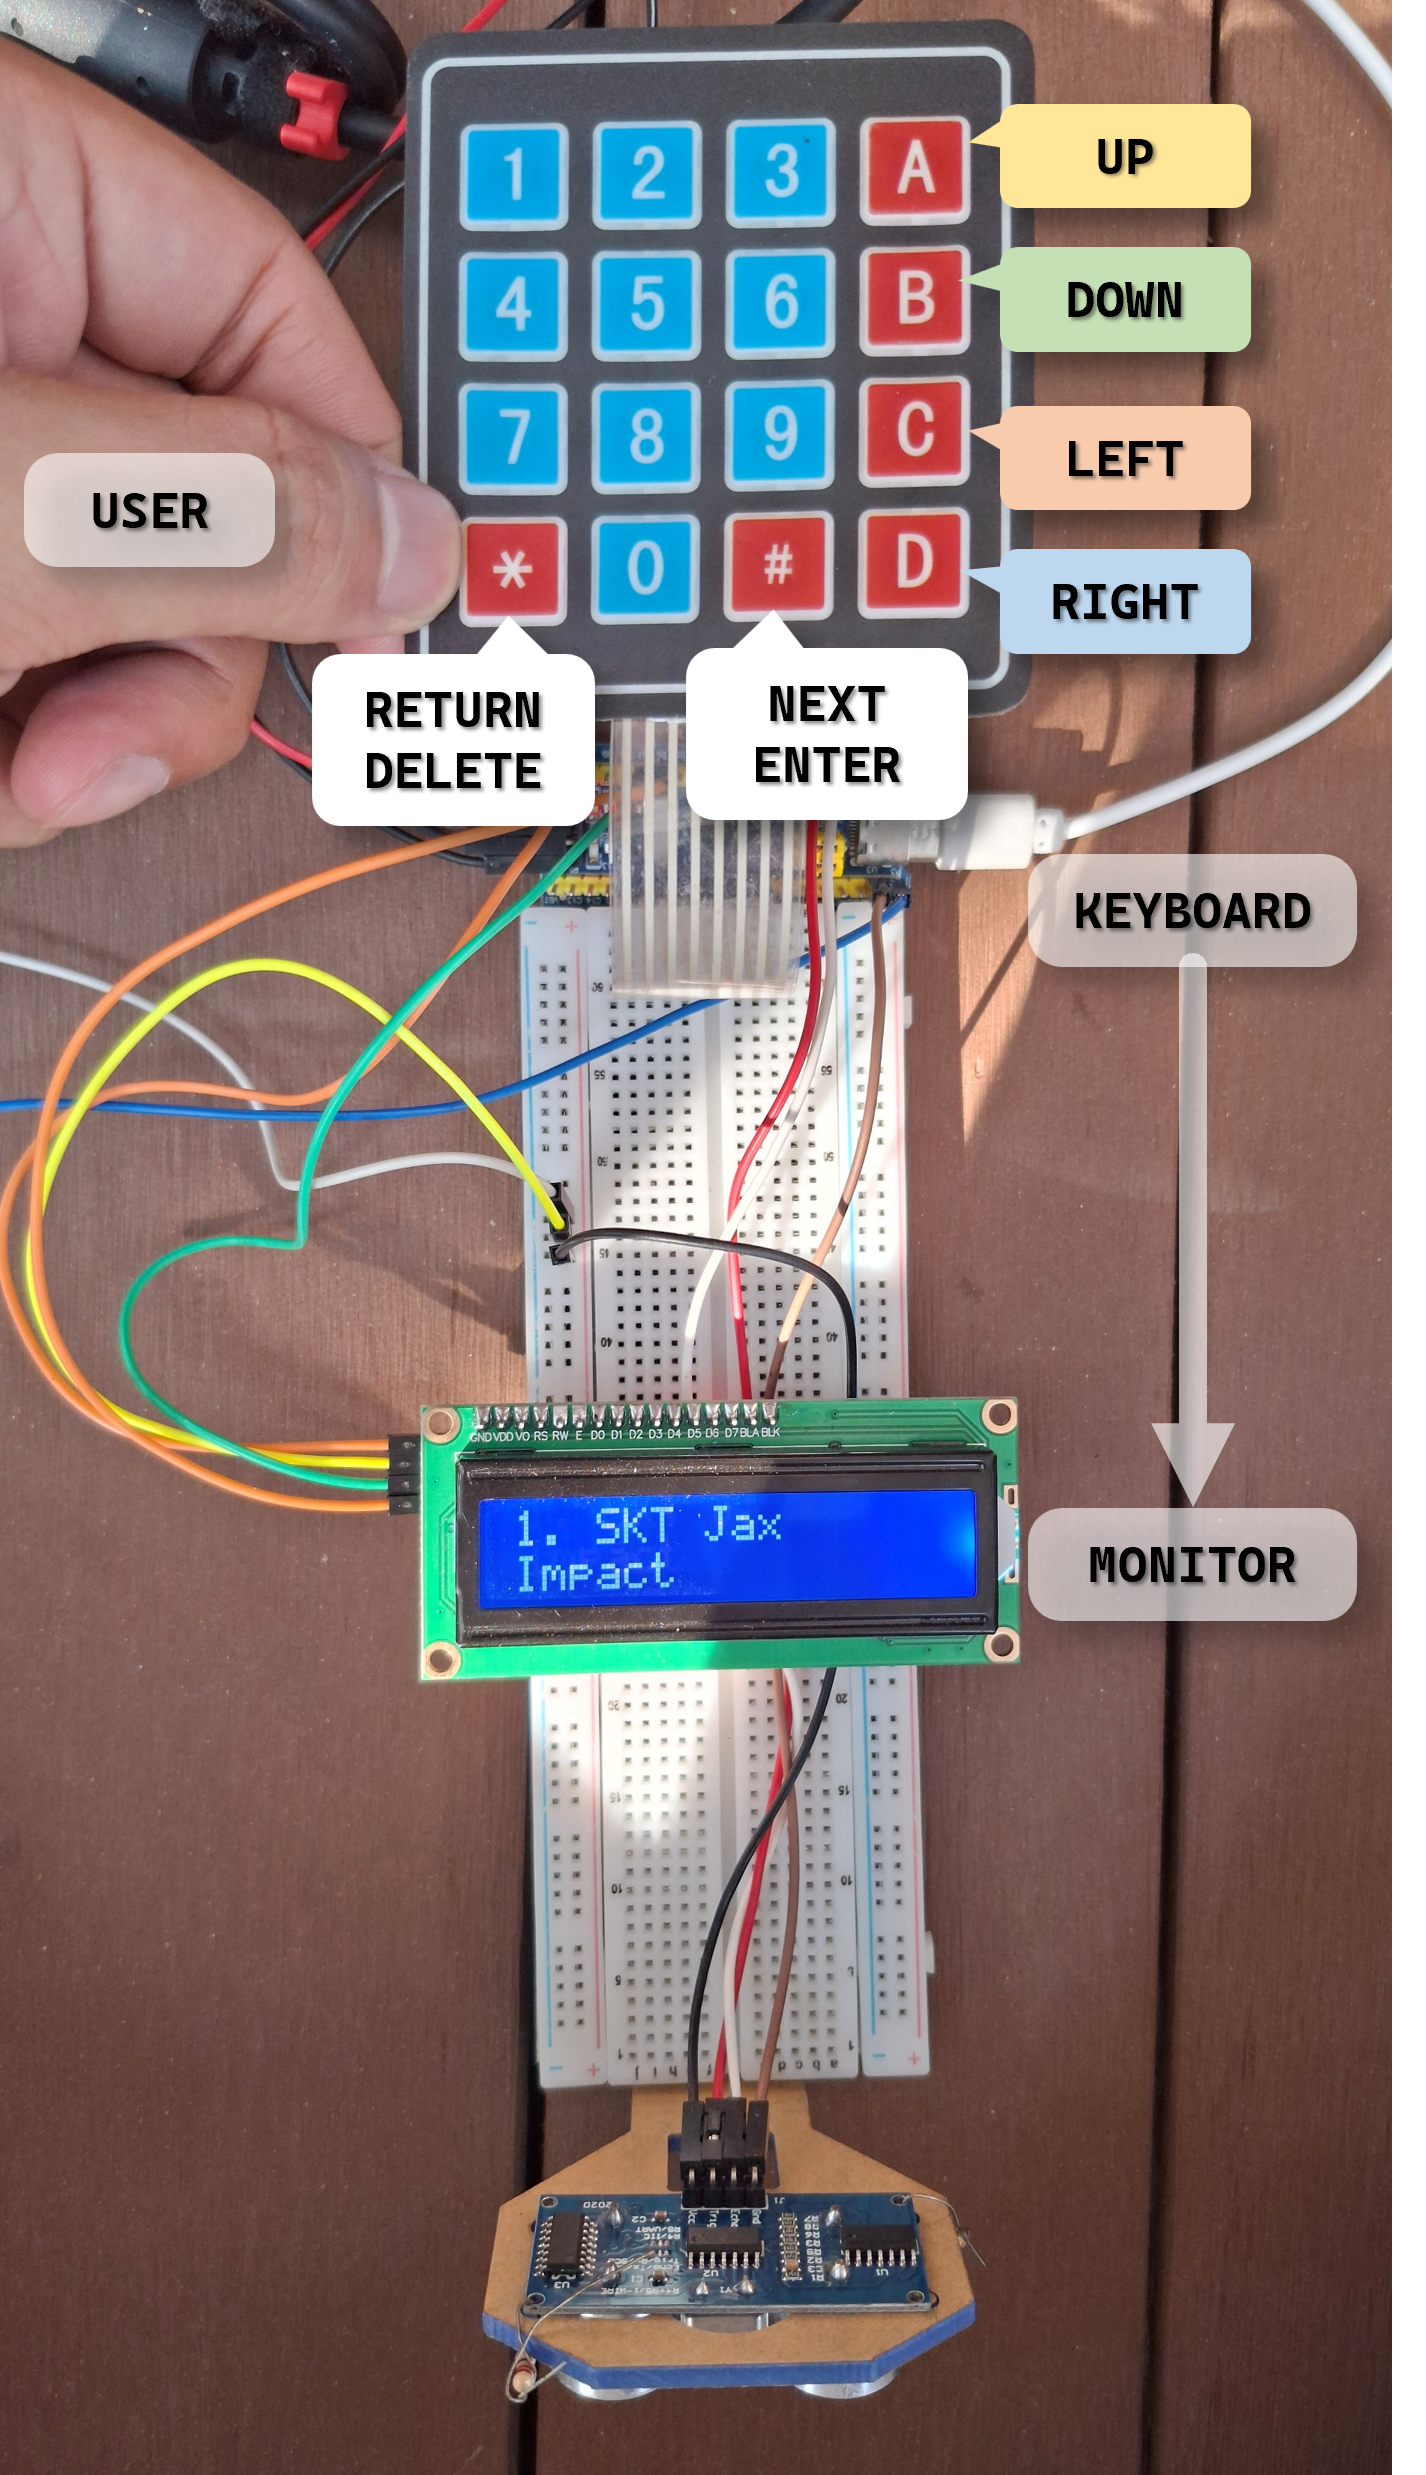
\includegraphics[width=\textwidth]{../Pictures/quickDemo_2.png}
        \caption{Demo vận hành hệ thống - Phần 2}
        \label{fig:demo_2}
    \end{subfigure}
    \caption{Trình diễn vận hành Máy bán hàng tự động}
    \label{fig:system_demo}
\end{figure}

\subsubsection{Kịch bản 1: Mua hàng Thành công}

\textbf{Trạng thái Ban đầu:} Hệ thống nhàn rỗi trong chế độ WAIT\_SENSOR

\begin{enumerate}[leftmargin=*]
    \item Khách hàng tiếp cận trong phạm vi 20cm, hệ thống phát hiện sự hiện diện trong 3 giây
    \item LCD hiển thị: "WELCOME TO DEMON KING STORE"
    \item Sau 3 giây, danh sách sản phẩm xuất hiện: "1. SKT Jax" / "Impact"
    \item Khách hàng nhấn 'D' năm lần để điều hướng đến sản phẩm \#6
    \item LCD hiển thị: "6. SKT Renekton" / "Marin"
    \item Khách hàng nhấn '\#' để xem chi tiết
    \item LCD hiển thị: "Available: 9" / "Price: 30000 \#6"
    \item Khách hàng nhấn '\#' lần nữa để xác nhận chọn
    \item LCD hiển thị: "ENTER QUANTITY" / "(1 TO 9):"
    \item Khách hàng nhập '2' cho hai đơn vị
    \item Khách hàng nhấn '\#' để xác nhận
    \item LCD hiển thị: "AMOUNT TO PAY" / "60000 VND" (trong 3 giây)
    \item LCD chuyển sang: "INSERT MONEY:" / (khu vực nhập ở giữa)
    \item Khách hàng nhập '50000' và nhấn '\#'
    \item LCD hiển thị: "REMAINING:" / "10000 VND" (trong 3 giây)
    \item LCD trở lại: "INSERT MONEY:"
    \item Khách hàng nhập '10000' và nhấn '\#'
    \item LCD hiển thị: "PAYMENT SUCCESS" / "CHANGE: 0 VND"
    \item Sau 3 giây: "THANKS FOR SUP" / "DEMON KING STORE"
    \item Kho hàng được cập nhật: Số lượng SKT Renekton giảm từ 9 xuống 7
    \item Hệ thống trở lại chế độ chọn sản phẩm
\end{enumerate}

\textbf{Tổng Thời gian Giao dịch:} Khoảng 45 giây

\subsubsection{Kịch bản 2: Xử lý Hết hàng}

\begin{enumerate}[leftmargin=*]
    \item Khách hàng điều hướng đến sản phẩm có số lượng 0
    \item Nhấn '\#' để xem chi tiết
    \item LCD hiển thị: "Available: 0" / "Price: 20000 \#1"
    \item Khách hàng nhấn '\#' để thử mua
    \item LCD ngay lập tức hiển thị: "OUT OF STOCK" / "CHOOSE ANOTHER"
    \item Sau 3 giây hoặc bất kỳ lần nhấn phím nào, trở lại chi tiết sản phẩm
    \item Khách hàng có thể nhấn '*' để trở lại danh sách sản phẩm
\end{enumerate}

\subsubsection{Kịch bản 3: Điều chỉnh Kho hàng Quản trị}

\begin{enumerate}[leftmargin=*]
    \item Từ chọn sản phẩm, quản trị viên nhấn phím 'R'
    \item LCD hiển thị: "ENTER PASSWORD"
    \item Quản trị viên nhập "070596" (hiển thị là *****)
    \item Sau 6 chữ số: "SUCCESS LOG IN" / "ADMIN MODE"
    \item Sau 3 giây: Danh sách sản phẩm xuất hiện
    \item Quản trị viên điều hướng đến sản phẩm mong muốn sử dụng 'U'/'D'
    \item Nhấn '\#' để vào chế độ điều chỉnh
    \item LCD hiển thị: ">>>Avail: 9" / "Price: 30000"
    \item Quản trị viên nhấn 'R' ba lần để tăng số lượng lên 12 (hiển thị lỗi ở mức tối đa 9)
    \item Nhấn 'D' để chuyển sang điều chỉnh giá
    \item LCD hiển thị: "Avail: 9" / ">>>Price: 30000"
    \item Quản trị viên nhấn 'R' năm lần để tăng giá thêm 5000 VND
    \item LCD hiển thị: "Avail: 9" / ">>>Price: 35000"
    \item Quản trị viên nhấn '\#' để lưu
    \item LCD hiển thị: "COMPLETE UPDATE" (trong 1.5 giây)
    \item Trở lại chọn sản phẩm trong chế độ quản trị
    \item Quản trị viên nhấn '*' sau đó '\#' để thoát chế độ quản trị
    \item Hệ thống trở lại chế độ khách hàng bình thường
\end{enumerate}

\subsection{Độ tin cậy Hệ thống}

Tất cả các đường dẫn lỗi được kiểm thử thành công:

\begin{itemize}[leftmargin=*]
    \item Đầu vào số lượng không hợp lệ bị từ chối chính xác và nhắc thử lại
    \item Số tiền thanh toán không hợp lệ kích hoạt thông báo lỗi và cho phép sửa chữa
    \item Điều kiện hết hàng ngăn chặn mua hàng và hướng dẫn người dùng đến các lựa chọn thay thế
    \item Các kịch bản thời gian chờ đưa hệ thống về trạng thái an toàn
    \item Chế độ quản trị tự động đăng xuất hoạt động chính xác sau 60 giây không hoạt động
    \item Thực thi giới hạn 5 lỗi ngăn chặn vòng lặp thử lại vô hạn
\end{itemize}

\newpage
\section{Đề xuất cho Công việc Tương lai}

While the current implementation successfully demonstrates embedded vending machine concepts, several enhancements could expand functionality and commercial viability.

\subsection{Màn hình Lớn hơn}

\textbf{Trạng thái Hiện tại:} LCD ký tự 16×2 giới hạn hiển thị thông tin.

\textbf{Cải tiến Đề xuất:}
\begin{itemize}[leftmargin=*]
    \item Nâng cấp lên LCD đồ họa (128×64 hoặc 320×240 pixel)
    \item Màn hình màu TFT với giao diện cảm ứng
    \item Hiển thị hình ảnh sản phẩm, thông tin dinh dưỡng, khuyến mãi
    \item Hỗ trợ đa ngôn ngữ với các biểu tượng đồ họa
\end{itemize}

\textbf{Lợi ích:} Cải thiện trải nghiệm người dùng, giảm thời gian làm quen, trình bày thương hiệu tốt hơn, tính năng hỗ trợ truy cập.

\subsection{Mở rộng Dung lượng Kho hàng}

\textbf{Trạng thái Hiện tại:} 16 sản phẩm bị giới hạn bởi điều hướng hiển thị và bộ nhớ.

\textbf{Cải tiến Đề xuất:}
\begin{itemize}[leftmargin=*]
    \item EEPROM ngoài (I2C/SPI) cho cơ sở dữ liệu kho hàng mở rộng
    \item Hỗ trợ 100+ sản phẩm với điều hướng dựa trên danh mục
    \item Lưu trữ thêm siêu dữ liệu sản phẩm (mô tả, hình ảnh, ngày hết hạn)
    \item Hiện thực truy vấn kiểu cơ sở dữ liệu cho tìm kiếm sản phẩm
\end{itemize}

\textbf{Cách tiếp cận Kỹ thuật:} AT24C256 (32KB EEPROM) hoặc lớn hơn, cấu trúc menu phân cấp, hệ thống phân loại sản phẩm.

\subsection{Hỗ trợ Đa ngôn ngữ}

\textbf{Trạng thái Hiện tại:} Giao diện chỉ tiếng Anh.

\textbf{Cải tiến Đề xuất:}
\begin{itemize}[leftmargin=*]
    \item Tùy chọn tiếng Việt, tiếng Anh và các ngôn ngữ khác
    \item Menu chọn ngôn ngữ khi khởi động hoặc qua chế độ quản trị
    \item Cấu trúc bảng chuỗi cho quản lý dịch thuật hiệu quả
    \item Hỗ trợ Unicode cho các ký tự không phải ASCII
\end{itemize}

\newpage
\section{Kết luận}

\subsection{Thành tựu Dự án}

Dự án này đã thiết kế và hiện thực thành công một hệ thống máy bán hàng tự động toàn diện sử dụng vi điều khiển STM32F103C8T6. Hệ thống hoàn chỉnh thể hiện ứng dụng thực tế của các khái niệm hệ thống nhúng và đạt được tất cả các mục tiêu chính:

\begin{itemize}[leftmargin=*]
    \item \textbf{Tích hợp Phần cứng Hoàn chỉnh:} Giao tiếp thành công vi điều khiển với màn hình LCD, bàn phím ma trận, cảm biến siêu âm và bộ nhớ Flash, tạo ra một hệ thống nhúng đầy đủ chức năng.
    
    \item \textbf{Hiện thực Máy trạng thái Mạnh mẽ:} Phát triển một FSM 19 trạng thái quản lý các luồng giao dịch phức tạp, xử lý lỗi và các chức năng quản trị với hành vi xác định.
    
    \item \textbf{Lưu trữ Dữ liệu Bền vững:} Hiện thực lưu trữ không bay hơi sử dụng bộ nhớ Flash nội với xác thực số ma thuật, đảm bảo dữ liệu kho hàng tồn tại qua các chu kỳ nguồn.
    
    \item \textbf{Trình điều khiển Ngoại vi Tùy chỉnh:} Tạo các trình điều khiển hiệu quả cho giao tiếp LCD I2C bit-banged, quét bàn phím chống rung và đo khoảng cách siêu âm dựa trên bộ định thời.
    
    \item \textbf{Xử lý Lỗi Toàn diện:} Hiện thực xác thực đầu vào, quản lý thời gian chờ, bộ đếm lỗi và cơ chế phục hồi đảm bảo độ tin cậy của hệ thống và hoạt động thân thiện với người dùng.
    
    \item \textbf{Tự động Phát hiện Khách hàng:} Đạt được hoạt động tự chủ với phát hiện sự hiện diện của khách hàng dựa trên cảm biến siêu âm và lọc nhiễu 3 giây.
    
    \item \textbf{Quản trị An toàn:} Cung cấp chế độ quản trị được bảo vệ bằng mật khẩu với bảo mật dựa trên thời gian chờ cho quản lý kho hàng.
\end{itemize}

\subsection{Ứng dụng Thực tế}

Mặc dù được phát triển như một dự án giáo dục, hệ thống thể hiện các khái niệm áp dụng cho máy bán hàng tự động thương mại và tự động hóa bán lẻ:

\begin{itemize}[leftmargin=*]
    \item Tự động phát hiện khách hàng giảm tiêu thụ năng lượng
    \item Theo dõi kho hàng cho phép trí tuệ kinh doanh
    \item Xử lý lỗi đảm bảo hoạt động liên tục
    \item Chế độ quản trị hỗ trợ bảo trì tại hiện trường
    \item Thiết kế mô-đun tạo thuận lợi cho mở rộng tính năng
\end{itemize}

Kiến trúc có thể được thích ứng cho các kịch bản bán lẻ tự động khác nhau bao gồm máy bán hàng truyền thống, ki-ốt bán vé, hệ thống cho thuê và tủ khóa thông minh.

\subsection{Lời kết}

Dự án máy bán hàng tự động đã đạt được thành công các mục tiêu thiết kế và hiện thực một hệ thống nhúng toàn diện thể hiện tích hợp phần cứng, điều khiển máy trạng thái, lưu trữ dữ liệu bền vững và tương tác người dùng. Hệ thống hoạt động tin cậy, xử lý lỗi một cách duyên dáng và cung cấp giao diện trực quan cho cả khách hàng và quản trị viên.

Ngoài các thành tựu kỹ thuật, dự án đã cung cấp kinh nghiệm quý báu về phương pháp thiết kế hệ thống nhúng, tích hợp phần cứng-phần mềm và giải quyết vấn đề dưới các ràng buộc tài nguyên. Kiến trúc mô-đun và tài liệu kỹ lưỡng đảm bảo hệ thống có thể phục vụ như một nền tảng cho các cải tiến trong tương lai và mục đích giáo dục.

Các kỹ năng phát triển qua dự án này—lập trình vi điều khiển, giao tiếp ngoại vi, thiết kế hệ thống thời gian thực và gỡ lỗi có hệ thống—có thể áp dụng trực tiếp cho phát triển hệ thống nhúng chuyên nghiệp trong tự động hóa công nghiệp, điện tử tiêu dùng và các ứng dụng IoT.

\newpage
\section{Thông tin Dự án}

\subsection{Kho lưu trữ Dự án}

Mã nguồn dự án, tài liệu và tài nguyên có sẵn tại:

\begin{itemize}[leftmargin=*]
    \item \textbf{Kho lưu trữ GitHub:} \url{https://github.com/1172005thinh/VendingMachine}
    \item \textbf{Cấu trúc Dự án:} Thư mục VendingMachine/ chứa tất cả các tệp nguồn
    \item \textbf{Tài liệu:} README.md với hướng dẫn thiết lập
\end{itemize}

\subsection{Tác giả}

\subsubsection{Nhóm Dự án}

Dự án này được phát triển bởi ba sinh viên từ Trường Đại học Bách Khoa - ĐHQG-HCM (HCMUT):

\begin{table}[H]
\centering
\begin{tabular}{|l|p{8cm}|}
\hline
\textbf{Tên} & \textbf{Đóng góp} \\
\hline
\textbf{Nguyễn Hưng Thịnh} & 
\begin{itemize}[leftmargin=*, nosep, after=\strut]
    \item Tích hợp phần cứng và thiết kế mạch
    \item Kiểm thử và gỡ lỗi hệ thống
    \item Chuẩn bị tài liệu
    \item Quan lý dự án và phối hợp nhóm
    \item Quay video trình diễn và soạn thảo báo cáo cuối cùng
\end{itemize} \\
\hline
\textbf{Lê Thế Lộc} & 
\begin{itemize}[leftmargin=*, nosep, after=\strut]
    \item Phát triển trình điều khiển bàn phím
    \item Hệ thống quản lý kho hàng
    \item Các hoạt động bộ nhớ Flash
    \item Thiết kế kiến trúc hệ thống
    \item Phát triển trình điều khiển cảm biến
\end{itemize} \\
\hline
\textbf{Trần Doãn Hoàng Lâm} & 
\begin{itemize}[leftmargin=*, nosep, after=\strut]
    \item Thiết kế và hiện thực máy trạng thái hữu hạn
    \item Hiện thực hệ thống bộ định thời
    \item Thiết kế giao diện người dùng
    \item Thực hiện, soạn kịch bản trình diễn
\end{itemize} \\
\hline
\end{tabular}
\end{table}

\subsubsection{Tổ chức}

\textbf{Trường Đại học Bách Khoa - ĐHQG-HCM (HCMUT)}

\begin{itemize}[leftmargin=*]
    \item Khoa Khoa học và Kỹ thuật Máy tính
    \item Bộ môn Đồ án Thiết kế Luận lý
    \item Địa chỉ: 268 Lý Thường Kiệt, Quận 10, Thành phố Hồ Chí Minh, Việt Nam
    \item Website: \url{https://www.hcmut.edu.vn/}
\end{itemize}

\subsubsection{Thông tin Khóa học}

\begin{itemize}[leftmargin=*]
    \item \textbf{Khóa học:} Đồ án Thiết kế Luận lý
    \item \textbf{Năm học:} 2025 - 2026
    \item \textbf{Thời gian Dự án:} Tháng 09/2025 - Tháng 12/2025
    \item \textbf{Ngày Hoàn thành:} \today
\end{itemize}

\subsection{Lời cảm ơn}

Các tác giả xin bày tỏ lòng biết ơn đến:

\begin{itemize}[leftmargin=*]
    \item Các cố vấn khoa về hướng dẫn các nguyên tắc thiết kế hệ thống luân lý
    \item Cộng đồng mã nguồn mở về các ví dụ mã và hỗ trợ khắc phục sự cố
\end{itemize}

\subsection{Giấy phép và Sử dụng}

Dự án này được phát triển cho mục đích giáo dục như một phần của khóa học tại HCMUT. Mã nguồn và tài liệu được cung cấp cho:

\begin{itemize}[leftmargin=*]
    \item Tham khảo giáo dục và học tập
    \item Nghiên cứu và học tập học thuật
    \item Trình diễn hệ thống nhúng phi thương mại
    \item Phát triển và cải tiến thêm
\end{itemize}

Đối với các ứng dụng thương mại hoặc các tác phẩm phái sinh, yêu cầu ghi công thích hợp cho các tác giả gốc và tổ chức.

\vspace{2cm}

\begin{center}
\rule{0.8\textwidth}{0.5pt}

\textit{Báo cáo này được biên soạn vào \today}

\textit{Trường Đại học Bách Khoa - ĐHQG-HCM}

\textit{Hệ thống Máy bán hàng Tự động - Đồ án Thiết kế Luận lý}

\rule{0.8\textwidth}{0.5pt}
\end{center}

\end{document}
